\chapter{فیلتر کالمن}

\section{؟}

برای توسعه این سامانه، ابتدا باید مدل یا متدولوژی توسعه آن مشخص می‌شد؛ با توجه به نیازمندی‌های این پروژه، ماهیت کسب و کاری آن و با استناد به سازوکاری بنام فیلتر بوهم و ترنر(با عنوان نمودار راداری)، این پروژه از مدل توسعه چابک  پیروی خواهد کرد. در توضیح، این نمودار 5 شاخصه اصلی‌ دارد که شامل نوع بازار کسب‌وکار، تعداد افراد تیم، سطح توانمندی افراد، مقدار تغییر نیازمندی‌ها در طول زمان و میزان تاثیر مخرب در صورت شکست پروژه می‌باشد.\cite{reqeng}\\

 با توجه به این 5 شاخص و با توجه به طبیعت پرتغییر نیازمندی‌های این پروژه، بهترین مدل برای توسعه آن، مدل توسعه افزایشی  بوده است و از بین متدولوژی ‌های آن، اسکرام  بدلیل سازماندهی و اولویت‌بندی مناسب نیازمندی‌های عملکردی سامانه، بهترین انتخاب خواهد بود. البته نکته قابل توجه در زمینه استفاده از اسکرام در این پروژه، یک نفره بودن آن است. در واقع متدولوژی‌های مانند اسکرام راهکارهایی نیز برای مدیریت تیم‌ها ارائه می‌دهند، اما در انجام این پروژه فقط از آن دسته استانداردها و راهکارهایی از اسکرام تبعیت شده که در مدیریت پروژه فردی نیز کاربرد خواهد داشت و معتبر خواهد بود.\\
 
پس از انتخاب مدل، نیازمندی‌ها بطور دقیق‌تری استخراج شدند و در ادامه، سامانه به چند زیر سیستم تقسیم شده و پس از اولویت‌بندی آن‌ها عملیات طراحی آغاز گردید.

از دیدگاه سطح بالا و با توجه به موارد گفته شده در قسمت‌های قبلی، مهم‌ترین بخشی که باید طراحی آن زودتر از بقیه انجام می‌شد، سامانه اصلی (باطن\footnote{\lr{Backend}}  سامانه) بود. برای پیاده‌سازی زیرسیستم‌ها، باید پشته نرم‌افزاری مورد استفاده مشخص می‌شد که اینکار با بررسی جوانب سامانه طراحی شده و ویژگی‌های هر پشته‌ی ممکن برای پیاده‌سازی آن، انجام شد.\\

در روال پیاده‌سازی، باید توجه ویژه‌ای به بحث آزمون ‌پذیری سامانه می‌شد تا بتوان در آینده از آن بطور موثرتری نگهداری کرد. برای آزمون سامانه، از برخی مجموعه تست‌های واحد و برخی تست‌های سطح سیستم استفاده شده است.

\newpage

%\subsection{ابزار مدیریت فرآیند}

برای نگهداری انباشته‌ی وظایف\footnote{\lr{Backlog}} و همچنین کنترل روال توسعه و تنظیم زمان شروع و پایان هر وظیفه در آن، از ابزارهای مختلفی می‌توان استفاده کرد. در این پروژه از ابزار بسیار معروف جیرا\footnote{\lr{Jira}} ساخته‌ی شرکت اطلسیان\footnote{\lr{Atlassian}} استفاده شده است. البته جایگزین‌هایی مانند ابزار ترلو\footnote{\lr{Trello}} (که ساخته دیگر همین شرکت است) یا ابزارهای ایرانی مانند سون‌تسک\footnote{\lr{SevenTask}} نیز وجود داشتند.\cite{jira}\\

طبق روال اسکرام در ابتدا در قسمت انباشت وظایف (مانند \cref{fig:jira1})،‌ تعداد زیادی از استوری\footnote{\lr{Story}}(داستان)های کاربر اضافه شدند. هرکدام از این داستان‌ها یکی از ویژگی‌های عملکردی یا غیرعملکردی سامانه را برای یک نقش کاربر خاص مشخص می‌کنند. در نوشتن این داستان‌ها سعی شده است که استاندارد جملات آن مطابق اسکرام رعایت شود.

طبق این استاندارد، جملات داستان‌ها باید به شکل "بعنوان یک ...، می‌خواهم که ...، تا بتوانم ...". در قسمت اول نقش کاربر موردنظر نوشته می‌شود؛ در قسمت دوم، عملکرد موردنظر سامانه و در قسمت سوم هدفی که آن کاربر از انجام عملکرد ذکر شده به دنبال تحقق آن است بیان می‌شود. این هدف بسیار مهم است، زیرا تا زمانی‌که با کیفیت مطلوب برآورده نشود، حتی می‌تواند نشان دهنده نقص نیازمندی‌های نوشته شده و کامل نبودن همین داستان‌های نوشته شده کاربر باشد؛ همچنین این اهداف، منبع خوبی برای ایجاد طرح آزمون‌های سطح سیستم هستند.

\begin{figure}[H]
	\centering
	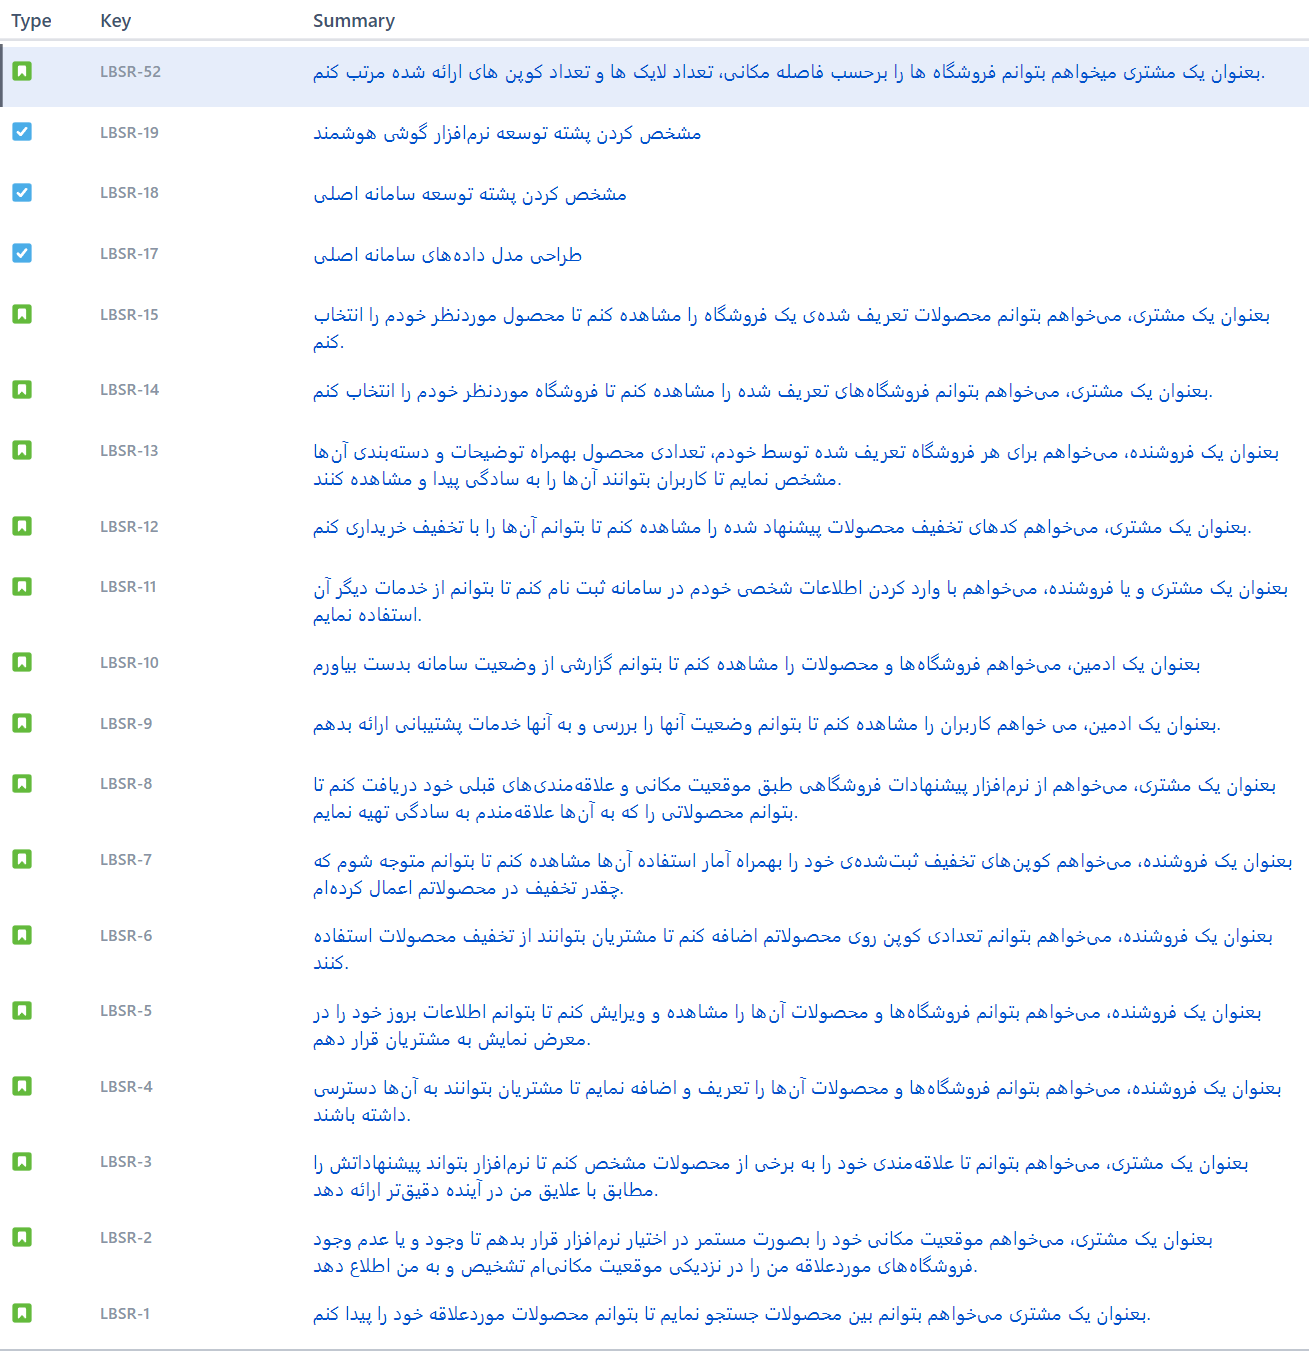
\includegraphics[scale=0.65]{jira1}
	\caption{بخشی از انباشته‌ی وظایف در جیرا}
	\label{fig:jira1}
\end{figure}

با توجه به این‌که وظایف\footnote{\lr{Tasks}} مطرح در این سامانه اکثرا از دو بخش ظاهر و منطق تشکیل شده‌اند، حوزه پیاده‌سازی آن‌ها نیز متفاوت است و اکثر وظایف بخش ظاهر در نرم‌افزار کاربردی تلفن همراه هوشمند پیاده‌سازی می‌شود؛ درحالی‌که اکثر وظایف بخش منطق و محاسبات در باطن\footnote{\lr{Backend}} سامانه (همان سامانه اصلی) پیاده‌سازی خواهد شد. بنابراین، این موارد بایستی از تقدم و تاخر دقیقی پیروی کنند تا در پیاده‌سازی آن‌ها وقفه ایجاد نشود.

\newpage

تحقق هر داستان کاربر، نیازمند اقداماتی در طراحی و پیاده‌سازی خواهد بود. برای اینکه از لحاظ زمانی انجام یک پروژه قابل پیش‌بینی باشد، برای هرکدام از این داستان‌های کاربر بایستی عددی تحت عنوان امتیاز آن\footnote{\lr{Story Point}} تعیین شود. این امتیاز درواقع واحد زمانی پیش‌بینی شده برای تحقق هر داستان کاربر است که بطور نسبی (نسبت به بقیه داستان‌ها) تخمین زده می‌شود. 

\begin{figure}[H]
	\centering
	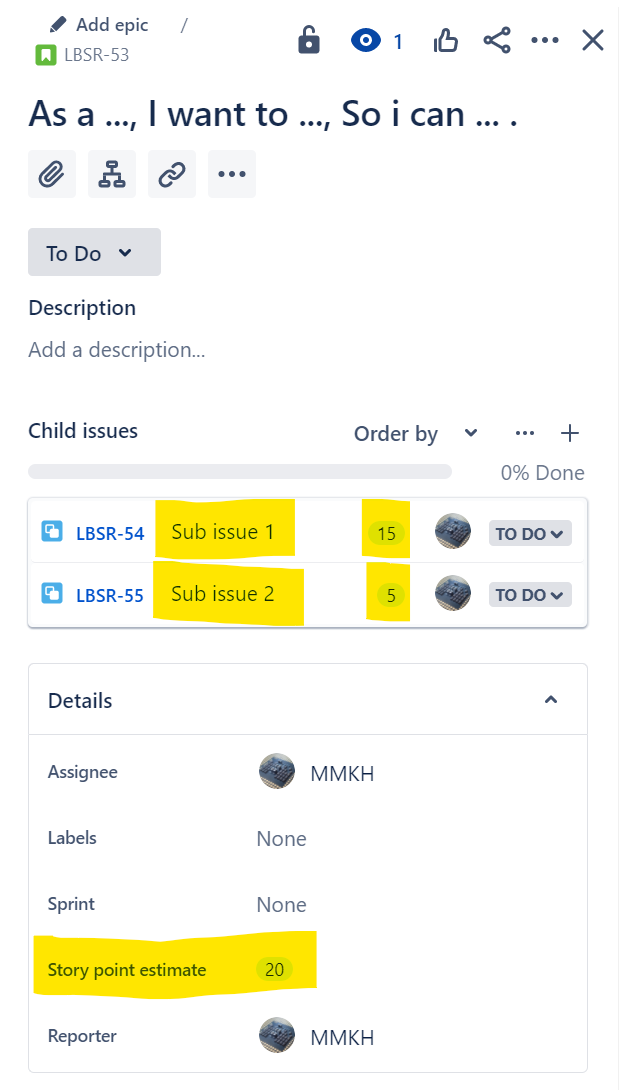
\includegraphics[scale=0.7]{jira2}
	\caption{زیروظیفه‌ها و امتیاز زمانی وظایف در جیرا}
	\label{fig:jira2}
\end{figure}

\newpage

%\section{طراحی مدل داده‌ها}

%\subsection{طرح ساده شده}

پس از تعیین و انتخاب روش‌های مدیریت پروژه و شروع تعریف وظایف، اولین قدم طراحی مدل داده‌ها\footnote{\lr{ِData Model}}ی سامانه بود. برای این‌کار مدل‌ها با معماری مختلفی درنظر گرفته شد، اما درنهایت آن مدلی که بیشترین سطح تودرتو بودن داده‌ها را بهمراه داشت انتخاب شد؛ جلوتر در همین سند، دلیل این انتخاب از نظر فنی توضیح داده خواهد شد. در توضیح \cref{fig:datamodel}، این نمودار از استانداردهای ای‌آر\footnote{\lr{ER‌  Diagram}} پیروی نمی‌کند؛ زیرا پیاده‌سازی این مدل از طریق پایگاه‌داده‌های رابطه‌ای انجام نخواهد شد.

\begin{figure}[H]
	\centering
	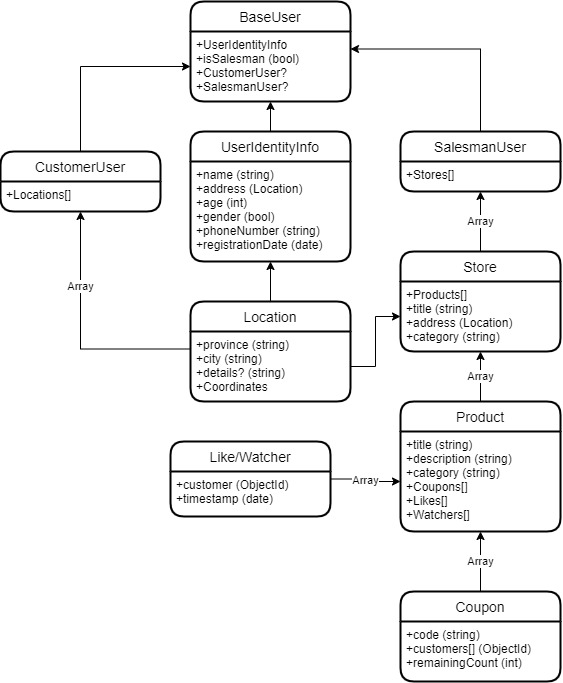
\includegraphics[scale=0.6]{datamodel}
	\caption{مدل داده‌های ساده شده سامانه}
	\label{fig:datamodel}
\end{figure}

\newpage

%\subsection{شرح مدل داده‌ها}

همان‌طور که در \cref{fig:datamodel} مشاهده می‌شود، شی اصلی در این مدل، شی \lr{BaseUser} است که نماینده هر کاربر از این سامانه می‌باشد. در ادامه 4 خصوصیت داخلی این شی را توضیح خواهیم داد:

\begin{enumerate}
	\item \lr{UserIdentityInfo}: این شی، شامل مشخصات فردی هر کاربر می‌باشد که خودش از 6 خصوصیت داخلی تشکیل شده است:
	\begin{enumerate}
		\item \lr{name}: این شی شامل نام و نام خانوادگی کاربر می‌شود (که نام را با \lr{fname} و نام خانوادگی را با \lr{lname} نگهداری می‌کند)،
		
		\item \lr{address}: این شی شامل آدرس محل زندگی کاربر می‌شود. بطورکلی هر آدرسی در این سامانه از شی \lr{Location} استفاده می‌کند که خودش شامل 4 خصوصیت زیر است:
		\begin{enumerate}[label=\arabic*.]
			\item \lr{Province}: نشان‌دهنده استان آدرس داده شده است،
			
			\item \lr{City}(یا \lr{Township} در پیاده‌سازی): نشان‌دهنده شهر آدرس داده شده است،
			
			\item \lr{Details}(یا \lr{Extra} در پیاده‌سازی): نشان‌دهنده جزئیات اضافی آدرس داده شده است،
			
			\item \lr{Coordinates}: که نماینده یک مختصات جغرافیایی است و شامل یک آرایه 2 عضوی‌ست. عضو اول مقدار \lr{longitude} و عضو دوم مقدار \lr{latitude} است،
		\end{enumerate}
		
		\item \lr{Age}(یا \lr{BirthYear} در پیاده‌سازی): نشان‌دهنده سن کاربر است؛ نکته مهم در مورد این خصوصیت، نیازمندی آن به بروزرسانی دائمی‌ست (زیرا دائما زمان و عمر افراد در حال گذشتن است!). برای حل این مشکل و عدم نیاز به بروزرسانی دائمی این خصوصیت، از \lr{BirthYear} استفاده شده که صرفا سال تولد کاربر را به شمسی نگهداری می‌کند و هر جایی از سامانه که به سن نیاز بود، بصورت درلحظه\footnote{\lr{Realtime}} سن کاربر محاسبه می‌شود،
		
		\item \lr{Gender}: این خصوصیت،‌ جنسیت کاربر را مشخص می‌کند،
		
		\item \lr{PhoneNumber}: شامل شماره تلفن همراه کاربر می‌شود که از طریق پیامک نیز احراز هویت شده است،
		
		\item \lr{RegistrationDate}: در این خصوصیت، شی زمان ثبت‌نام کاربر نگهداری می‌شود،
	\end{enumerate}

	\item \lr{isSalesman}: این خصوصیت،‌ نوع حساب کاربر را مشخص می‌کند؛ به این معنا که کاربر موردنظر فروشنده است و یا خریدار،
	
	\item \lr{CustomerUser}: این شی، شامل آرایه‌ای از موقعیت‌های کاربر خریدار است که بصورت تناوبی ثبت شده است،
	
	\item \lr{SalesmanUser}: درون این شی که برای کاربران فروشنده است، فقط یک خصوصیت قرار دارد:
	\begin{enumerate}
		\item \lr{Stores}: این شی شامل آرایه‌ای از فروشگاه‌های ثبت‌شده‌ی فروشنده می‌شود. هر فروشگاه شامل 4 خصوصیت است:
		\begin{enumerate}[label=\arabic*.]
			\item \lr{Products}: این شی شامل آرایه‌ای از محصولات ثبت‌شده‌ی فروشنده برای این فروشگاه می‌شود. هر محصول شامل 6 خصوصیت است:
				\begin{enumerate}
					
					\item \lr{Title}: این خصوصیت عنوان محصول را نشان می‌دهد،
					
					\item \lr{Category}: این خصوصیت گروه دسته‌بندی محصول را نشان می‌دهد،
					
					\item \lr{Description}: این خصوصیت توضیحات اضافی محصول را شامل می‌شود،
					
					\item \lr{Coupons}: این خصوصیت، کوپن‌های تخفیف را نمایندگی می‌کند و شامل آرایه‌ای از آن‌ها برای هر محصول می‌شود،
					
					\item \lr{Likes, Watchers}: این دو خصوصیت، علاقه‌مندی‌ها و زیرنظرداشتن‌های محصولات را نگهداری می‌کنند،
					
					
				\end{enumerate}
			
			\item \lr{Title}: این خصوصیت عنوان فروشگاه را نشان می‌دهد،
			
			\item \lr{Category}: این خصوصیت گروه دسته‌بندی فروشگاه را نشان می‌دهد،
			
			\item \lr{Address}: این خصوصیت محل فیزیکی فروشگاه را نشان می‌دهد که در آن از شی \lr{Location} استفاده شده که پیش‌تر توضیح داده شد،
				
		\end{enumerate}
	\end{enumerate}

\end{enumerate}

\newpage

%\section{طراحی مورد کاربرد}

مهم‌ترین مرحله تولید یک سامانه نرم‌افزاری همزمان با طراحی مدل داده‌های آن، طراحی نمودار مورد کاربرد\footnote{\lr{UseCase Diagram}} است. در \cref{fig:ucdiag} نمودار مورد کاربرد این سامانه که در طرح پروژه تصویب شده نیز موجود بوده‌است مشاهده می‌شود. البته این موردهای کاربرد صرفا بعنوان یک حداقل از این سامانه مطرح شده‌اند و درآینده موردهای کاربرد این سامانه می‌تواند بسیار گسترده‌تر و پیچیده‌تر شود.

\begin{figure}[H]
	\centering
	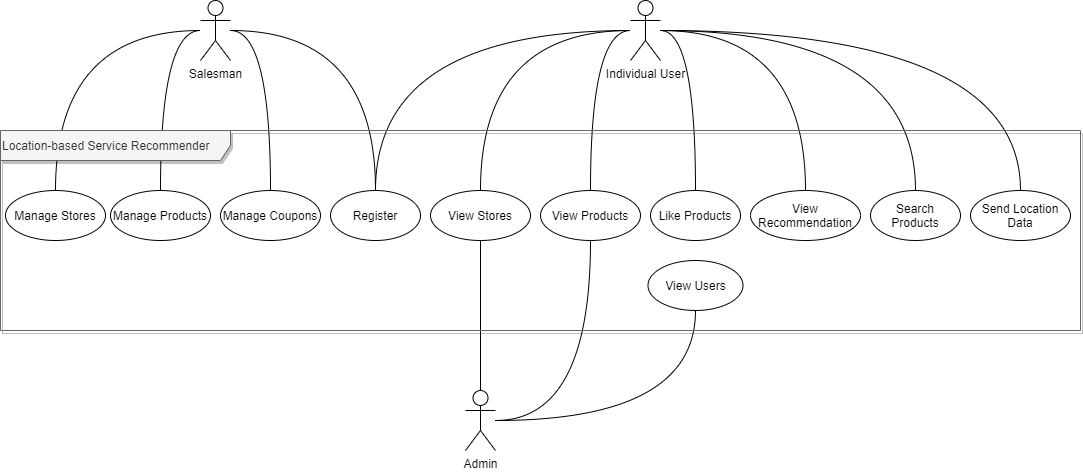
\includegraphics[scale=0.4]{ucdiag}
	\caption{موردهای کاربرد سامانه}
	\label{fig:ucdiag}
\end{figure}

بطورکلی سه گروه استفاده‌کننده از این سامانه وجود خواهند داشت:
\begin{enumerate}
	\item \lr{Salesman}: همان فروشندگان هستند که با ایجاد فروشگاه و محصول و ارائه کدهای تخفیف برای محصولات خود، داده موردنیاز جهت پیشنهاد به خریداران را برای سامانه فراهم می‌کنند.
	\item \lr{Individual User}: خریداران یا همان کاربران عادی این سامانه هستند که با اعلام علاقه‌مندی خود به محصولات مختلف، از سامانه پیشنهاداتی برای خرید محصولات متناسب با علاقه خود و همچنین متناسب با موقعیت مکانی لحظه‌ای خود دریافت می‌کنند. در پیاده‌سازی انجام شده به این گروه کاربران \lr{Customer} نیز گفته شده است.
	\item \lr{Admin}: مدیران، پشتیبانان و ناظران سامانه هستند که از طریق پنل نظارتی که دراختیارشان قرار می‌گیرد، می‌توانند از طریق وب اقدام به مشاهده لیست تمامی کاربران و اطلاعات آنان و اطلاعات تمام فروشگاه‌ها محصولات نمایند.
\end{enumerate}

\newpage

%\section{انتخاب پشته نرم‌افزاری}

همان‌طور که در بخش آخر فصل مقدمه توضیح داده شد، در این پروژه از پشته نرم‌افزاری زیر استفاده شده است:

\begin{itemize}
	\item \lr{Node.js (+ Typescript)}
	\item \lr{Apollo (+ Express)}
	\item \lr{GraphQL}
	\item \lr{MongoDB}
	\item \lr{Mocha (+ Chai)}				
	\item \lr{React Native}
	\item \lr{ReactJS}
\end{itemize}

در ادامه دلیل انتخاب هر کدام از این موارد را بهمراه برخی از رقبا مطرح خواهیم کرد.

%\subsection{مونگو، بعنوان پایگاه داده}

برای پایگاه داده، بطورکلی می‌توان از بین \lr{SQL}های رابطه‌ای و \lr{NoSQL}ها انتخاب کرد. برای انتخاب نوع پایگاه داده، باید ابتدا مدل داده‌ها را طراحی کرد. بطورکلی اگر سازماندهی داده‌ها بصورت خطی باشد و لینک‌ها و ارتباطات زیادی با آی‌دی‌ها و کلیدها به یکدیگر داشته باشند (موجودیت‌های ضعیف کم و قوی زیاد)، مدل‌های رابطه‌ای بهتر هستند، و اگر بصورت تودرتو و عمیق (موجودیت‌های ضعیف زیاد و قوی کم) باشند، مدل‌های غیررابطه‌ای بهتر هستند.

علاوه بر این موضوع، در انتخاب پایگاه داده مسائل دیگری نظیر قابلیت مقیاس‌پذیری عمودی و افقی نیز مطرح است و بویژه برای کاربرد این سامانه، مقیاس‌پذیری افقی بسیار حائز اهمیت خواهد بود. اکثر پایگاه‌های داده رابطه‌ای از مقیاس‌پذیری افقی مناسبی برخوردار نیستند، البته نسخه‌هایی از \lr{PostgreSQL} از این نوع مقیاس‌پذیری پشتیبانی خوبی دارند، اما بطورکلی پایگاه‌های داده \lr{NoSQL} در این موضوعات پیشرو هستند.

با توجه به دو مورد بالا، انواع \lr{NoSQL} انتخاب بهتری برای کاربرد ما خواهند بود. از بین این پایگاه‌های داده، پایگاه‌داده مونگو بیشترین پشتیبانی و جامعه استفاده‌کنندگان را دارد و به همین دلیل بنظر می‌آید بهترین انتخاب باشد.

%\subsection{نودجی‌اس، بعنوان چارچوب اصلی سامانه}

برای پیاده‌سازی بدنه اصلی سامانه، زبان‌ها و چارچوب‌های بسیاری وجود دارند که برخی از آن‌ها عبارت‌اند از:
\begin{itemize}
	\item پایتون\footnote{\lr{Python}}
	\item پی‌اچ‌پی\footnote{\lr{PHP}}
	\item نودجی‌اس\footnote{\lr{Node.js}}
	\item جاوا\footnote{\lr{Java}}
	\item ای اس پی (دات نت)\footnote{\lr{ASP.net}}
	\item گو\footnote{\lr{Go}}
\end{itemize}

برخی از این زبان‌ها مانند جاوا و ای‌اس پی و تا حدی پی‌اچ‌پی، اساسا برای نرم‌افزارهای چابک خیلی مناسب نیستند و بیشتر برای پروژه‌های دولتی و بسیار بزرگ مناسب‌اند و انعطاف‌پذیری آن‌ها در برابر تغییرات سریع نیست و برای پیاده‌سازی اولیه یک سامانه زمان بیشتری به نسبت بقیه زبان‌ها نیاز خواهند داشت.

از بین زبان‌های نوشته شده، گو بهترین عملکرد را خواهد داشت، اما مشکل اصلی آن کوچک بودن نسبی جامعه استفاده‌کنندگان فعلی آن به نسبت دیگر موارد است. همچنین استفاده چابک از پایتون نیز بیشتر برای پیاده‌سازی نمونه‌اولیه\footnote{\lr{Prototype}} مناسب خواهد بود، زیرا عملکرد آن بخصوص از لحاظ مقیاس‌پذیری افقی، به نسبت نودجی‌اس ضعیف‌تر است. بنابراین با توجه به کلیات مطرح شده، نودجی‌اس بهترین انتخاب خواهد بود.

ارائه‌دهندگان سرویس وب معروفی که تحت زبان جاواسکریپت و چارچوب نودجی‌اس قابل استفاده هستند، شامل این موارد هستند:
\begin{itemize}
	\item اکسپرس\footnote{\lr{Express}}
	\item هَپی\footnote{\lr{Hapi}}
	\item کوآ\footnote{\lr{Koa}}
\end{itemize}

از جهت سرعت عملکرد، حجم، جامعه استفاده‌کنندگان و سربار، بهترین انتخاب اکسپرس خواهد بود. البته دلیل دیگری نیز برای این انتخاب وجود دارد که به استاندارد مورد استفاده در ارتباط بین سامانه اصلی و نرم‌افزار تلفن‌های هوشمند و پنل تحت وب مدیران مربوط می‌شود، که همان گرف‌کیوال و کتابخانه آپولو است که در ادامه توضیح داده می‌شود.\cite{express}

%\subsection{گرف‌کیوال و آپولو، بعنوان ارتباط‌دهنده}

دو استاندارد بسیار معروف برای ارتباط بین سامانه اصلی و سامانه‌های کاربری مطرح است:

\begin{itemize}
	\item رِست\footnote{\lr{RESTful API}}
	\item گرف‌کیوال\footnote{\lr{GraphQL}}
\end{itemize}

که البته مورد اول تاکنون بسیار معروف‌تر بوده است.

گرف‌کیوال (که در فصل دوم بطور مفصل توضیح داده شد)، یک استاندارد ارتباطی است که در آن فقط از درخواست پُست\footnote{\lr{POST}} با بدنه داده‌های مورد درخواست استفاده می‌شود و سرور تمام موارد خواسته شده را پر کرده و در جواب همان درخواست، می‌فرستد. به این صورت که تمام موارد درخواستی فقط به یک رفت و برگشت نیاز خواهند داشت. البته این روش چالش‌هایی نیز دارد اما در کل برای کاربردهایی که حجم اینترنت مصرفی در آن‌ها حائز اهمیت است، و یا برای کاربردهایی که ساختارداده‌های آن‌ها بصورت عمیق و تودرتو باشد، عموما استفاده از رِست بصرفه نخواهد بود.

برای استفاده از گرف‌کیوال، کتابخانه آپولو معروف‌ترین کتابخانه است و مورد استفاده قرار خواهد گرفت. این کتابخانه در سمت سامانه اصلی پیاده‌شده تحت نودجی‌اس، از خدمات‌دهنده وب اکسپرس استفاده می‌کند.\cite{apollo}



%\subsection{اتوماسیون استقرار و آزمون}

برای استقرار خودکار، از داکر استفاده شده است که درحال حاضر بهترین روش برای توسعه چابک سامانه‌های چندبخشی‌ست (و البته می‌توان گفت که چندان گزینه دیگری هم موجود نیست). برای تست، با توجه به این‌که سامانه اصلی با نودجی‌اس نوشته شده، از ابزار موکا و چای استفاده خواهد شد که امکان ایجاد تست‌های بی‌دی‌دی\footnote{\lr{BDD}} و تی‌دی‌دی\footnote{\lr{TDD}} را به ما می‌دهد و برای اجرای آن‌ها بصورت خودکار نیز سازوکارهایی دارد.

برای اتصال این موارد به یکدیگر و اجرای خودکار و یکپارچه آن‌ها، از قابلیت‌های \lr{CI/CD} ارائه دهندگان سرویس گیت (مانند گیت‌هاب\footnote{\lr{GitHub}}، گیت‌لب\footnote{\lr{GitLab}} و بیت‌باکت\footnote{\lr{BitBucket}}) استفاده شده است.


%\subsection{ری‌اکت، بعنوان چارچوب نرم‌افزار کاربردی}

در بخش نرم‌افزار کاربردی، با توجه به این‌که بدنبال ساخت نرم‌افزار کاربردی گوشی هوشمند هستیم، و ظاهر و منطق این نرم‌افزارها توسط یک چارچوب پیاده‌سازی می‌شوند، گزینه‌های زیر موجود هستند که پس از معرفی به ذکر مشکلات هر کدام خواهیم پرداخت:

\begin{itemize}
	\item ایجاد نرم‌افزار کاربردی با زبان‌های بومی هر سیستم‌عامل (جاوا/کاتلین برای اندروید، سوییفت/آبجکتیو-سی برای آی او اس)
	\item استفاده از چارچوب چندسکوی ری‌اکت نیتیو
	\item استفاده از چارچوب چندسکوی زامارین\footnote{\lr{Xamarin}}
	\item ایجاد نرم‌افزار بصورت تحت وب، با ابزارهایی مانند فون‌گپ\footnote{\lr{PhoneGap}} و... .
\end{itemize}

مورد اول بسیار زمان‌بر است و بدلیل ماهیت چابک این پروژه و بطورکلی بازار فعلی نرم‌افزارهای گوشی‌های موبایل، بصرفه نخواهد بود. مورد دوم، نسبت به مورد سوم از این جهت نقص دارد که فقط روش اجرای در لحظه\footnote{\lr{JIT (Just In Time)}} را پشتیبانی می‌کند و نه جلوتر از زمان\footnote{\lr{AOT (Ahead Of Time)}} که در نهایت منجر به عملکرد کندتری خواهد شد. مورد سوم متاسفانه بطور کامل رایگان نیست و همچنین اخیرا از لحاظ پشتیبانی کاربران و جامعه کاربری، از مورد دوم جا مانده است و همچنین کتابخانه‌های آماده کمتری برای آن موجود است. مورد چهارم نیز مناسب اپلیکیشن‌هایی با تاکید بر کاربرد موقعیت مکانی و سرویس اعلان\footnote{\lr{Notification Service}} نیست. بنابراین بهترین انتخاب، استفاده از ری‌اکت می‌باشد.

\newpage

%\section{طراحی اجزای پروژه}

%\subsection{محدوده اجزا}

\begin{figure}[H]
	\centering
	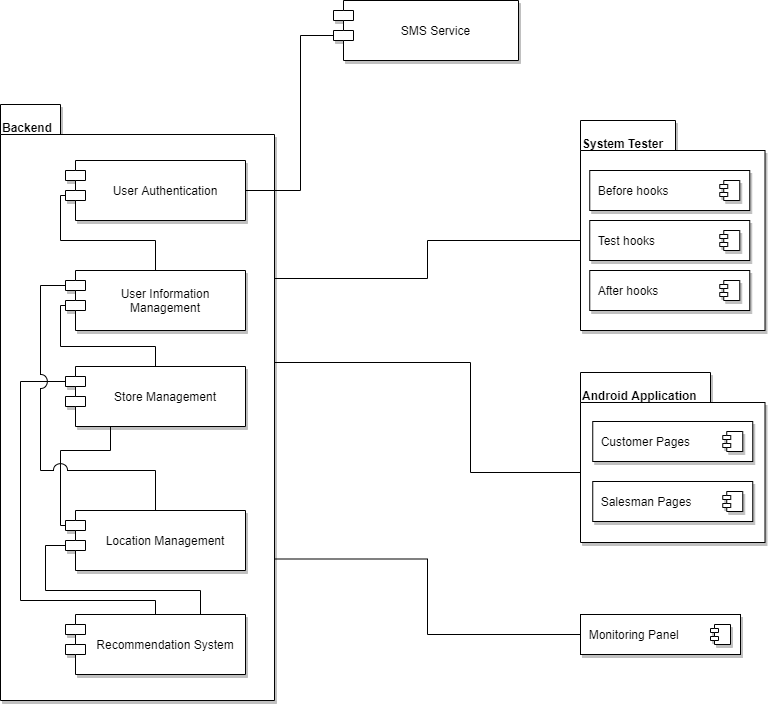
\includegraphics[scale=0.6]{cdiag}
	\caption{محدوده اجزا و نحوه ارتباط آن‌ها}
	\label{fig:cdiag}
\end{figure}

همان‌طور که در \cref{fig:cdiag} نمایش داده شده است، سامانه اصلی همان \lr{Backend} است؛ نرم‌افزار کاربردی تلفن هوشمند، \lr{Android Application}، پنل نظارتی مدیران سامانه \lr{Monitoring Panel} و بخشی از سامانه که برای آزمون سامانه اصلی مورد استفاده قرار می‌گیرد و شامل مجموعه‌ای از آزمون‌های واحد و آزمون‌های سطح سیستم است، توسط \lr{System Tester} نمایندگی شده است.

\newpage

بخشی تحت عنوان \lr{SMS Service} نیز در این نمودار وجود دارد که می‌تواند رابط برنامه‌نویسی کاربردی\footnote{\lr{API}} هر ارائه‌دهنده خدمات پیامکی باشد. از این بخش جهت ارسال پیام‌کوتاه کدتایید ثبت‌نام و ورود و برای احراز هویت شماره تلفن همراه کاربران استفاده می‌شود. در سامانه پیاده‌سازی شده محل اتصالات و الحاق این ارائه‌دهنده طراحی شده اما درحال حاضر جهت سادگی کار توسعه، به هیچ سامانه پیامکی متصل نیست (و کدتایید تمام کاربران بصورت پیشفرض مقدار شش صفر خواهد بود).

در ادامه، بخش های درون \lr{Backend} را توضیح خواهیم داد:

\begin{enumerate}
	\item \lr{User Authentication}: شامل اجزائی می‌شود که در فرآیند احزارهویت و حفظ امنیت حساب کاربران نقش دارند؛
	\item \lr{User Information Management}: شامل اطلاعات هویتی و شخصی هر کاربر می‌شود، مانند نام، سن، آدرس و ...؛
	\item \lr{Store Management}: شامل تمام اطلاعات ثبتی فروشندگان از فروشگاه‌هایشان بهمراه تمام محصولات، دسته‌بندی‌ها و کدهای تخفیف می‌شود؛
	\item \lr{Location Management}: این بخش که در پیاده‌سازی بخش بزرگی از آن در بخش‌های دیگر ترکیب شده است، شامل عملکردهای مرتبط با موقعیت مکانی می‌شود (مانند تبدیل مختصات به آدرس و ...)؛
	\item \lr{Recommendation System}: این قسمت که بیشتر بعنوان یک رابط\footnote{\lr{Interface}} درنظر گرفته شده‌است، وظیفه بررسی علاقه‌مندی‌های پیشین و ایجاد پیشنهادات مختلف با توجه به موقعیت مکانی است که در فصل اول این سند به آن پرداخته شده بود.
\end{enumerate}

\newpage

%\subsection{معماری پیاده‌سازی}

در بخش قبلی، کل سامانه اصلی را از لحاظ وظایف بخش‌های مختلف آن به چند دسته تقسیم کردیم. اما باید توجه داشته باشیم این دسته‌بندی صرفا برای فهم بهتر موضوع و برنامه‌ریزی و هدف‌گذاری بهتر روال توسعه است و لزوما پیاده‌سازی با این تقسیم‌بندی انجام نمی‌شود (و در عمل هم نشده است). درواقع برای پیاده‌سازی این سامانه، بهتر است از معماری تقریبا یکپارچه\footnote{\lr{Monolithic}} استفاده شود؛ بجز مواردی مانند رابط پیامکی و رابط سیستم توصیه‌گر. 

البته طراحی انجام شده برای پشته\footnote{\lr{Stack}} و اجزای این پروژه، عملا امکان تبدیل آن به معماری ریزخدمت\footnote{\lr{Microservice}} را فراهم می‌کند؛ اما درحال حاضر این معماری صرفا به پیچیدگی‌های زائد مدیریت این سامانه می‌افزاید و برای پیاده‌سازی اولیه توصیه نمی‌شود.

همچنین، برای پیاده سازی سامانه اصلی سعی شده از یک سازوکار مشابه مدل-ظاهر-کنترل‌گر\footnote{\lr{MVC (Model-View-Controller)}} استفاده شود. در واقع بخش ظاهر سامانه اصلی به نرم‌افزار کاربردی این سامانه (از جمله نرم‌افزار تلفن‌های هوشمند و پنل مدیریتی) انتقال پیدا کرده است و در سامانه اصلی فقط اجزای مدل-کنترل‌گر وجود دارند.

در بخش نرم‌افزار کاربردی این سامانه، با توجه به این‌که از چارچوب ری‌اکت استفاده شده، از دیدگاه داده‌ها، از یک معماری تقریبا لایه‌ای استفاده شده است که چالش‌هایی را نیز به پیاده‌سازی اضافه کرده که در فصل بعدی به آن‌ها خواهیم پرداخت.

\newpage

%\subsection{ذخیره توصیفات امنیتی}

هر سامانه نرم‌افزاری، ویژگی‌های خاص خود را از نظر نیازمندی‌های امنیتی دارد. بسیاری از روش‌های رفع این نیازمندی‌ها که می‌توانند بسیار گسترده و متنوع نیز باشند، در یک سازوکار با یکدیگر مشترک هستند و آن، استفاده از توصیفات امنیتی برای رفع نیازمندی‌های امنیتی‌ست. توصیفات امنیتی\footnote{\lr{Security Descriptors}} شامل کلیدها، بلیت‌ها، رمزها،  قراردادهای امنیتی، پروتکل‌ها و... می‌شوند که روش‌های پاسخگویی به نیازهای امنیتی یک سامانه را مشخص می‌کنند. بنابراین این زیربخش به روش‌های تامین امنیت در این سامانه نمی‌پردازد؛ زیرا عمده این روش‌ها در بخش‌های خارج از پیاده‌سازی این سامانه (از جمله پایگاه‌داده مونگو، سامانه پیامکی و ...) اجرا شده است و این سامانه صرفا از آن‌ها استفاده خواهد کرد. بنابراین اولین چالش امنیتی سامانه اصلی این پروژه، حفظ توصیفات و مشخصات امنیتی مربوط به سازوکارهای امنیتی سامانه‌های بیرونی است.

برای ذخیره‌سازی توصیفات امنیتی سامانه (مانند رمز پایگاه داده و بلیت\footnote{\lr{Token}} رابط پیامکی) از سازوکار ویژه‌ای در این سامانه استفاده شده‌است. اغلب افرادی که پروژه‌های تحقیقاتی انجام می‌دهند، از این موضوع مهم غافل می‌شوند و توصیفات امنیتی را بصورت سخت‌کدشده\footnote{\lr{Hardcoded}} درون کدهای پیاده‌سازی خود می‌آورند و این موضوع متاسفانه در برخی شرکت‌هایی که اقدام به جذب کارآموز نیز می‌کنند مشاهده می‌شود و کارآموزان از همان روز اول به بخش مهمی از توصیفات امنیتی دسترسی خواهند داشت!


پس با توجه به اهمیت مضاعف اطلاعات موقعیت مکانی افراد، بایستی از توصیفات امنیتی (شامل کلیدها و رمزهایی که برای رمزنگاری اطلاعات استفاده می‌شوند) در این سامانه بخوبی محافظت شود و یکی از مواردی که باید رعایت شود، عدم حضور هیچ‌گونه توصیفات صریح امنیتی درون کد پیاده‌سازی شده است؛ درواقع به این معنا که اگر فرد یا افرادی به کد پیاده‌سازی شده دسترسی پیدا کردند، خطر مستقیمی از لحاظ توصیفات امنیتی سامانه را تهدید نکند (هرچند ممکن است بصورت غیرمستقیم و بدلیل نامناسب بودن سازوکار اصلی پیاده‌سازی شده که از این توصیفات استفاده می‌کند همچنان خود آن سازوکار تهدیدآمیز باشد که این موضوع مستقل از حفظ محرمانگی توصیفات امنیتی است). برای احراز امنیت این توصیفات، پس از تحقیق و بررسی بطورکلی 4 راه‌حل برای ذخیره توصیفات امنیتی شناخته شدند\cite{secrets}:

\begin{enumerate}
	\item استفاده از فایل، بدون رمزنگاری
	\item استفاده از فایل، با رمزنگاری متقارن\footnote{\lr{Symmetric Encyption}}
	\item استفاده از متغیرهای محیطی\footnote{\lr{Environment Variables}}، بدون رمزنگاری
	\item استفاده از متغیرهای محیطی، با رمزنگاری متقارن
\end{enumerate}

شاید در نگاه اول، انتخاب بین عدم رمزنگاری و رمزنگاری داده‌ها به جهت حفظ محرمانگی، بدیهی و رمزنگاری کردن داده‌ها منطقی‌تر باشد؛ اما در عمل اینطور نیست! اگر داده‌ها رمزنگاری شوند، برای گشودن رمز آن‌ها، نیازمند کلید خواهیم بود؛ حتی اگر رمزنگاری نامتقارن باشد، باز هم به کلید خصوصی رمزنگاری نیاز خواهیم داشت. مهم‌ترین نقطه‌ای که باید این رمزنگاری را بگشاید، سامانه اصلی است؛ پس کلید باید درون سامانه اصلی بصورت سخت‌کدشده نوشته شود! بنابراین اگر فردی به کدهای سامانه اصلی دسترسی داشته باشد (مثلا به فایل‌های سرور که کدها نیز جزئی از آن هستند)، قطعا کلیدها را نیز خواهد داشت و عملا اینکار تاثیر مثبتی ایجاد نمی‌کند. از طرفی، افراد مجازی که می‌خواهند مشخصات امنیتی را تغییر دهند،‌ باید همگی آن کلید را با خود حمل کنند و داشته باشند؛ و این فرآیند به خودی خود باعث پخش آن کلید می‌شود و اعتماد کاذبی که استفاده از اینگونه رمزنگاری ایجاد می‌کند، می‌تواند مخرب نیز باشد!

انتخاب بین متغیرهای محیطی و فایل، در وهله اول بستگی به محیط استقرار\footnote{\lr{Deployment}} دارد؛ برای مثال در یکی از محیط‌های ایرانی استقرار سکو بعنوان خدمت\footnote{\lr{PaaS (Platform as a Service)}} به نام دارکوب\footnote{\lr{Darkube}}\cite{darkube} که از ابزار کوبرنیتیز\footnote{\lr{Kubernetes}} و داکر\footnote{\lr{Docker}} برای استقرار خودکار استفاده می‌کند، امکان ایجاد فضای فایل مشترک بین چند ظرف مجازی\footnote{\lr{Container}} وجود ندارد. بنابراین اگر بخواهیم چنین سامانه‌ای را در این محیط مستقر و اجرا کنیم، مجبوریم از متغیرهای محیطی استفاده کنیم، چون دسترسی مستقیمی به فایل‌های آن وجود ندارد تا بتوان از روشی غیر از دریافت کدهای منبع از ابزارهای کنترل نسخه\footnote{\lr{Version Control}} (مانند گیت)، فایل‌های توصیفات امنیتی را پیش از اجرا به سامانه منتقل کرد. اما یک نکته بسیار مهم درمورد متغیرهای محیطی وجود دارد؛ محتویات این متغیرها توسط تمامی کتابخانه‌های سوم شخص\footnote{\lr{3rd Party libraries}} استفاده شده در کد سامانه قابل دسترسی هستند و این خودش می‌تواند نوعی آسیب امنیتی باشد! درست است که احتمالا وجود یک کتابخانه مخرب در بین مجموعه کتابخانه‌های استفاده شده در کد سامانه بسیار ناچیز است، اما وقتی از دیدگاه امنیت داده به یک موضوع نگاه می‌کنیم، نباید احتمالات ناچیز با اهمیت بالا را نادیده بگیریم.

با توجه به مطالبی که توضیح داده شد، بهترین انتخاب گزینه اول (فایل بدون رمزنگاری) خواهد بود. درواقع با این‌کار، هم کمترین تاثیر مخرب بر سرعت عملکرد سامانه ایجاد خواهد شد و هم بالاترین سطح امنیت تامین می‌گردد. البته همانطور که گفته شد، درصورتی می‌توان این روش را انجام داد که به فایل‌های محیط استقرار بصورت مستقل از ابزارهای کنترل نسخه دسترسی داشته باشیم و بتوان توصیفات را جداگانه به محیط استقرار منتقل کرد. همچنین اگر سامانه موردنظر ما از چند سرویس جدا تشکیل شده باشد، ولی این سرویس‌ها از توصیفات امنیتی یکسانی استفاده کنند، بهتر است از یک فضای فایل اشتراک‌گذاری شده\footnote{\lr{Shared Filesystem}} بین آن‌ها استفاده کرد. بنابراین محیط استقرار باید از این ویژگی نیز برای فضای فایل خود پیشتیبانی نماید و اگر امنیت پایدار در محرمانگی این توصیفات امنیتی اهمیت بالایی در طراحی ما دارد، باید از محیطی برای استقرار استفاده کرد که این ویژگی‌ها را احراز کند.

درنهایت، برای آزمایش این پروژه درحین توسعه و بصورت موقت، از سرویس دارکوب برای استقرار استفاده شده است که از ویژگی‌های گفته شده پشتیبانی نمی‌کند و موقتا از متغیرهای محیطی برای ذخیره مشخصات امنیتی استفاده شده است. اما برای استقرار نهایی و ورود به بازار این پروژه، حتما باید از محیط استقرار دیگری استفاده شود.

\newpage

%\subsection{فعالیت‌ها در سامانه}

در این‌جا صرفا برای توضیح بیشتر جزئیات پیاده‌سازی، سه فعالیت مهم که کاربران در این سامانه می‌توانند انجام بدهند را در قالب سه نمودار نمایش و توضیح خواهیم داد.

%\subsubsection{فعالیت ورود/ثبت‌نام کاربر}

در ابتدا با فعالیت ورود و ثبت‌نام کاربر شروع می‌کنیم:

\begin{figure}[H]
	\centering
	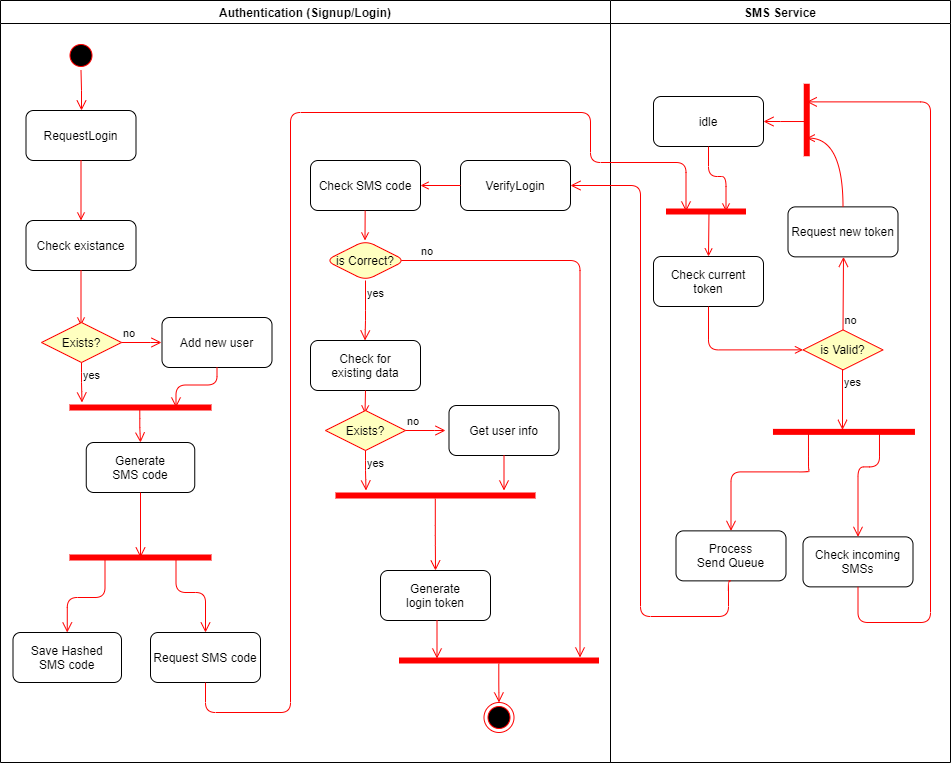
\includegraphics[scale=0.5]{adiag1}
	\caption{فعالیت ورود/ثبت‌نام کاربر}
	\label{fig:adiag1}
\end{figure}

آن‌چه در \cref{fig:adiag1} مشاهده می‌شود، روال طی شده برای ثبت‌نام و یا ورود هر دو گروه کاربران به سامانه است. برای احراز هویت از یک سرویس پیامکی استفاده خواهد شد که بصورت دوره‌ای باید بلیت آن از ارائه‌دهنده سرویس پیامکی دریافت شود تا در مواقع نیاز، درخواست ارسال پیامک به سمت سرویس پیامکی فرستاده شود.\\

امروزه در بسیاری از سامانه‌های خدمت‌رسانی برخط، روال ثبت‌نام با ورود مجدد تفاوت چندانی ندارد و درهنگام ثبت‌نام اولیه، صرفا اطلاعات هویتی اولیه‌ای دریافت می‌شود و در ادامه هیچ تفاوتی بین این دو روال وجود نخواهد داشت. در سامانه ما نیز چنین است و اگر کاربر برای بار اول وارد شود، صفحات اطلاعات اولیه هویتی و اطلاعات مکانی نمایش داده خواهد شد.

همان‌طور که پیش‌تر نیز گفته شد، روال ورود از دو مرحله تشکیل شده‌است:
\begin{enumerate}
	\item ورود شماره موبایل و درخواست شروع فرآیند احرازهویت شماره که در این نمودار تا مرحله ارسال پیامک را شامل می‌شود،
	\item دریافت کدفعالسازی ورود و احرازهویت که از طریق سامانه پیامکی ارسال شده است و مطابقت آن با کد ارسالی و مجوز ورود درصورت صحت آن که از مرحله \lr{VerifyLogin} به بعد است.
\end{enumerate}

برای جلوگیری از ورودهای غیرمجاز (حتی در صورت دسترسی مهاجم به پایگاه‌داده)، کد فعالسازی موقتی ایجاد شده در پایگاه‌داده بصورت درهم‌سازی‌شده\footnote{\lr{Hashed}} ذخیره می‌شود که در بلوک آخر بخش سمت چپ نمودار نیز قابل مشاهده است.

\newpage

%\subsubsection{فعالیت مشاهده فروشگاه‌ها}

نمودار این فعالیت در \cref{fig:adiag2} قابل مشاهده است:

\begin{figure}[H]
	\centering
	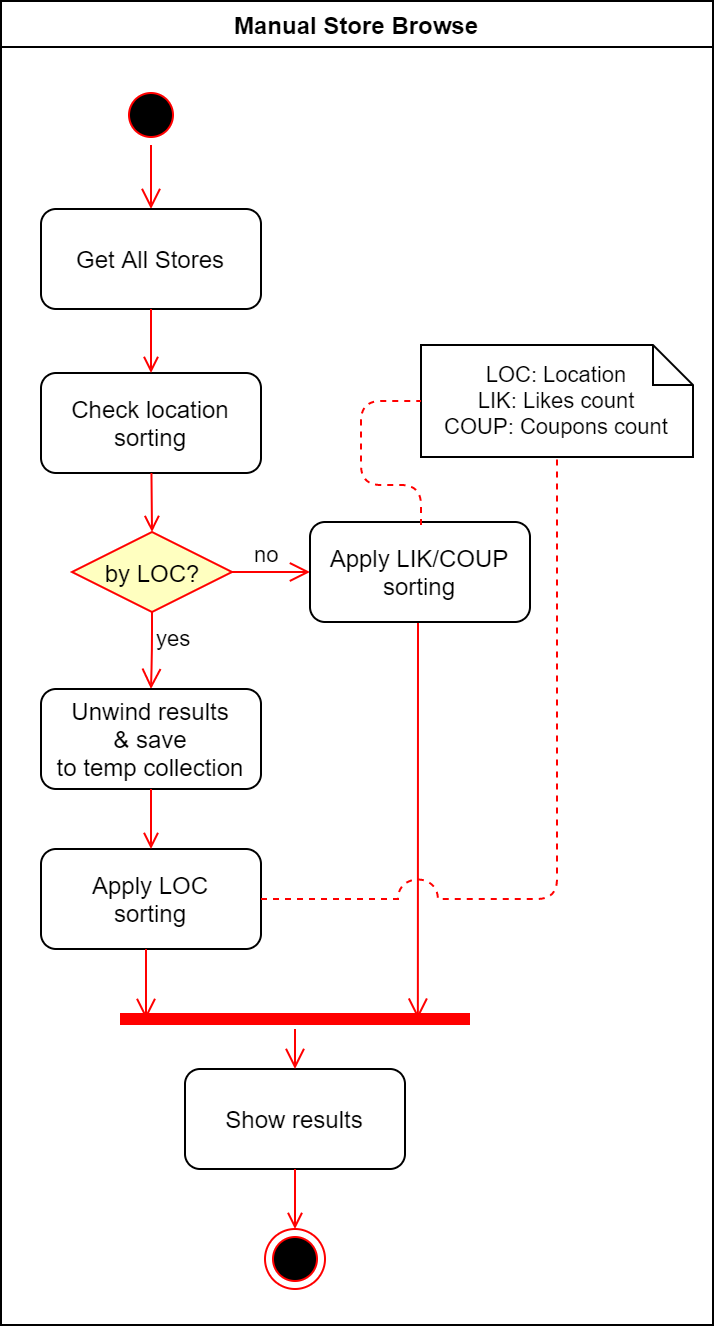
\includegraphics[scale=0.3]{adiag2}
	\caption{فعالیت مشاهده فروشگاه‌ها}
	\label{fig:adiag2}
\end{figure}

برای مشاهده فروشگاه‌ها، سه نوع مرتب‌سازی تعریف شده است:
\begin{enumerate}
	\item مرتب‌سازی بر اساس موقعیت مکانی؛‌ که در این نوع مرتب‌سازی بدلیل وجود چالش‌هایی که فصل بعد به آن خواهیم پرداخت، مراحل اضافه‌تری به نسبت انواع دیگر اجرا ‌می‌شوند که در نمودار نیز مشهود است،
	\item مرتب‌سازی بر اساس تعداد علاقه‌مندی ثبت شده،
	\item مرتب‌سازی بر اساس تعداد کوپن‌های تخفیف ارائه شده.
\end{enumerate}

درواقع اصلی‌ترین فعالیتی که برای مشاهده فروشگاه‌ها انجام می‌شود، عملیات مرتب‌سازی است که نیازمند اجرای محاسبات موقتی (مانند محاسبه حاصل جمع تعداد علاقه‌مندی‌های ثبت شده و یا کوپن‌های ارائه شده) پس از ارسال درخواست مشاهده فروشگاه‌ها است.

%\subsubsection{فعالیت دریافت پیشنهاد توسط کاربر}

\begin{figure}[H]
	\centering
	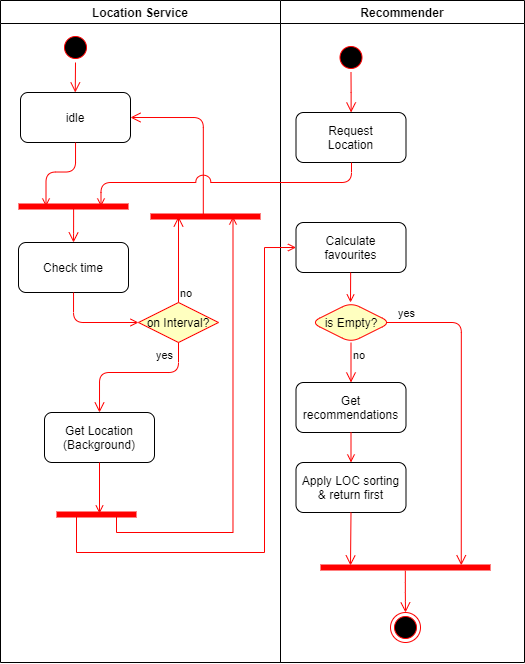
\includegraphics[scale=0.6]{adiag3}
	\caption{فعالیت دریافت پیشنهاد توسط کاربر}
	\label{fig:adiag3}
\end{figure}

این فعالیت شامل دو بخش کلی است؛ بخش اول که در سمت چپ نمودار \cref{fig:adiag3} مشاهده می‌شود، فعالیت ارائه پیشنهاد خودکار است. در واقع یک سرویس در پس‌زمینه\footnote{\lr{Background Service}} تلفن همراه کاربر بصورت دوره‌ای اقدام به اخذ موقعیت مکانی او و ارسال آن به سمت سامانه اصلی می‌کند؛ ادامه این فعالیت در بخش سمت راست انجام می‌پذیرد.

در بخش سمت راست نمودار \cref{fig:adiag2} که روال دریافت پیشنهاد از نرم‌افزار را نمایش می‌دهد، در ابتدای آن مرحله غیر خودکار دریافت موقعیت مکانی کاربر وجود دارد که در ادامه آن وارد بخش قبلی می‌شود تا موقعیت مکانی فعلی (یا قبلی) را برای کاربر دریافت نماید. پس از دریافت موقعیت مکانی، محاسبات مرتبط با علاقه‌مندی‌های کاربر از روی سوابق او انجام می‌شوند و درصورتی‌که محاسبات خروجی داشت و داده‌های موجود از سابقه کاربر برای محاسبه علاقه‌مندی‌ها کفایت می‌کرد، اقدام به پیش‌بینی مقدار علاقه‌مندی کاربر به محصولات و فروشگاه‌های دیگر می‌شود و درنهایت پس از مرتب‌سازی براساس نزدیکی به موقعیت مکانی فروشگاه‌ها (طبق موقعیت مکانی که در ابتدای این روال از کاربر دریافت شده بود)، نزدیک‌ترین فروشگاه به او پیشنهاد می‌شود.


